%%%%%%%%%%%%%%%%%%%%%%%%%%%%%%%%%%%%%%%%%%%%%%%%%%%%%%%%%%%%%%%%%%%%%%%%%%%%%%%%%%%%%%%%%
%%%%%%%%%%%%%%%%%%%%%%%%%%%%%%          TESTING PLAN         %%%%%%%%%%%%%%%%%%%%%%%%%%%%
%%%%%%%%%%%%%%%%%%%%%%%%%%%%%%%%%%%%%%%%%%%%%%%%%%%%%%%%%%%%%%%%%%%%%%%%%%%%%%%%%%%%%%%%%

\section{Testing Plan} % (15 points)
\label{sec:TestingPlan}
% Section Requirements:
% 1) Component and ground test plan
% 2) Flight test plan 

As mentioned in \cref{ssec:ManufacturingFlow} and shown in \cref{fig:plannedtiming,fig:manufacturingplan}, each of our design and build iterations culminate in testing.  Testing is divided into ground and flight testing. For all phases, we will start ground testing roughly a week after prototyping has commenced. We will perform formal flight tests near the end of each phase, in the week following the termination of the prototyping.
% {\color{BYUred}[NEED TO FLESH OUT DETAILS BELOW BASED ON THE SPECIFICS OF THE COMPETITION AND YOUR CONCEPTUAL DESIGN.  Also be sure to include details about what data you will gather and how you will use it.]}


%%%%%%%%%%%%%%%%%%%%%%%%%%%%
%%%% - Ground Testing - %%%%
%%%%%%%%%%%%%%%%%%%%%%%%%%%%
\subsection{Component/Ground Test Plan}
\label{ssec:GroundTestingPlan}
\begin{wrapfigure}[10]{R}{0pt}
	\centering
	\raisebox{0pt}[\dimexpr\height-2\baselineskip\relax]{ %NOTW: CHANGE THIS - VALUE TO SHIFT THE FIGURE UP INTO THE SECTION TITLE AREA IF YOU NEED TO.  OTHERWISE, COMMENT OUT THIS LINE
		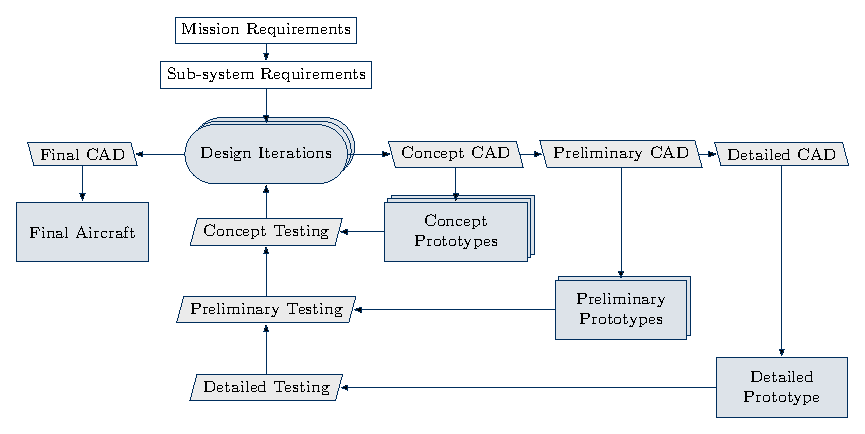
\includegraphics[width=0.6\textwidth]{manufacturing_flow}
	} %NOTE: IFF YOU COMMENT OUT THE \RAISEBOX LINE ABOVE, COMMENT OUT THIS LINE TOO.
	\caption{Iterative 3-phase development flow}
	\label{fig:manufacturingplan}
\end{wrapfigure}
\subsubsection{Phase 1} We began with shock sensor drop tests to understand how gentle our take-off, turning, landings, and drop-offs need to be. This allowed us to narrow down our payload manager concepts, and limit testing to only a few potential payload manager concepts, gathering data on ease of loading, simplicity of design, and dependability in order to finalize major design details.  We also brainstormed a variety of tests for our subsystems as described below.

\subsubsection{Phase 2} In our preliminary testing phase, we will be looking at more detailed payload manager prototypes, also taking into account speed in order to finalize our designs. A major component of this phase will be wind tunnel testing in the BYU 3'x4' open circuit wind tunnel.  For our propulsion system we will test across a full range of advance ratios using an RC Benchmark 1580 Dynamometer to validate the performance of, and make adjustments to, our selected propulsion system.  We will also examine the performance of a small variety of high lift configurations for our wing in order to validate our simulations of short takeoff/landing configurations, including gathering data on rotor-on-wing interactions (see \cref{fig:vpm}).  In addition to these wind tunnel tests, we will perform structural testing of our composite wing prototypes and other critical structures, including landing gear, gathering yield and failure data to apply appropriate safety factors to our final designs.  It should be noted that at the beginning of this phase, we will assemble and test the safety systems required in this year's competition rules.

\subsubsection{Phase 3} After finalizing our wing and tail manufacturing methods, we will need to test them in the wind tunnel again, this time gathering data on their aeroservoelastic behavior at high velocities in order to validate our structural design and manufacturing quality.  %We will also perform the required wing structural tests/demonstrations with a fully loaded aircraft.  
Finally,  we will do full system tests, performing dry runs of the ground mission as well as the on-ground components of FM3. This will allow us final tweaks on the design prior to our final competition build which we will similarly test with dry runs.


%%%%%%%%%%%%%%%%%%%%%%%%%%%%
%%%% - Flight Testing - %%%%
%%%%%%%%%%%%%%%%%%%%%%%%%%%%
\subsection{Flight Test Plan}
\label{ssec:FlightTestingPlan}

\subsubsection{Phase 1} We began our flight testing with a hand-launched, unpowered, uncontrolled glider.  Our primary goals for these tests were to validate our static stability and general structural calculations, as well as jump start the aeronautical intuition of our new team members. 

\subsubsection{Phase 2} In the preliminary phase of flight testing, we will begin with an unpowered, controlled, hand-launched glider to which we will add capabilities as our design progresses.  As our preliminary design progresses and after the completion of some of the wind tunnel testing described above, we will perform flight tests with a fully operational, powered, airframe, though without payload capabilities.  After adding propulsion capabilities to the airframe, we will utilize a flight controller as our main data acquisition device,  along with cameras, chronometers, and measuring tapes to complete all our testing regimens.
Our goal for the preliminary testing is to gather general flight data to validate our preliminary design simulations, record aircraft performance, and note any unexpected behavior in the aircraft dynamic responses before moving on to detailed design aspects and full system integration.

\subsubsection{Phase 3} As our detailed design prototype will be sufficient to compete if needed, our goal for the final testing phase will be to fly the complete mission sequence, allowing for any final fine-tuning of the design before building our competition aircraft. We will collect all the data required for a complete design report, again using primarily a flight controller and other on-board, data acquisition hardware.
